\chapter{Evaluation}

\section{Evaluation Method} 

 
\textbf{Dataset:} 
This database comprises 1511 quality annotated images based on 1511 source reference image patches that are subject to different distortion levels of compression. 
Differential mean opinion score (DMOS) for this dataset were computed for each pair, which is in the range 1 to 5.

\textbf{Evaluation Metrics:}
To evaluate the performances of the IQA algorithms, we used two standard measures, i.e., Spearman's rank order correlation coefficient (SRCC) and Pearson's linear correlation coefficient (PLCC).

\textbf{Experiment Setup:}
Both the experiments in this thesis are performed on HMII database.

For the first experiment, the purpose is to evaluate how well an objective metric agrees with subjective preferences of subjects. We carefully select the Mathlab implementations of 7 algorithms to predict object scores for the entire database. 

For the second one, different models are competed to find the best \enquote*{ground truth} predictor for patch quality. 
Results reported are based on the average performance of 10 folds cross-validation. Deep learning models converge after 50 epochs.   


\section{Experiment results}

\subsection{HMII Benchmark Analysis}

First, we evaluate the pairwise preference consistency using the classic correlation coefficients SRCC and PLCC,
as shown in Table \ref{tab:algos}. 
The SRCC and PLCC are
the average values for the distorted images of the same
reference image, and the top 2 correlation coefficient values are highlighted. 
We can see that the PSNR and UQI are poorly correlated
with human perceptual quality, and even contrary to subjective
results. This defective performance of PSNR is also mentioned in the work of Zhang \emph{et al.}\cite{Zhang2019} about Fine-Grained Quality Assessment. Although VSI combine the HVS features and achieve more
consistent results than PSNR in global image assessment, it is poorly correlated with human perceptual quality in fine-grained patch quality assessment.
For the two correlation coefficients, these IQA methods
shows quite similar characteristics. As a whole, FSIM achieves top 2 performance for all the cases and the SSIM achieves better performance with PLCC while SRSIM performs better with SRCC. 

\begin{table}[ht]
  \centering
  \begin{tabular}{|l|cc|cc|}
    \hline
    \multirow{2}{*}{} & \multicolumn{2}{c|}{ HMII (64x64) }      & \multicolumn{2}{c|}{ HMII (128x128) }    \\ \cline{2-5} 
    & PLCC           & SRCC           & PLCC           & SRCC           \\ \hline
    SSIM\cite{Wang2004}             & \textbf{0.785} & 0.787          & \textbf{0.795} & 0.797          \\
    RFSIM\cite{Zhang2010}             & 0.774          & 0.757          & 0.789          & 0.759          \\
    FSIM\cite{Zhang2011}              & \textbf{0.794} & \textbf{0.799} & \textbf{0.824} & \textbf{0.815} \\
    PSNR              & 0.200          & 0.737          & 0.194          & 0.752          \\
    UQI\cite{Wang2002}               & 0.023          & 0.621          & 0.012          & 0.589          \\
    VSI\cite{Zhang2014}               & 0.765          & 0.765          & 0.768          & 0.786          \\
    SRSIM\cite{Zhang2012}             & 0.777          & \textbf{0.803} & 0.718          & \textbf{0.803} \\ \hline
  \end{tabular}
  \caption{PLCC and SRCC for different IQA algorithms}
  \label{tab:algos}
\end{table}

In addition to visualize the objective score by the top 3 IQA algorithms, we plot the distributions of subjective scores and objective scores on a 2-D graph and also plot the fitted curve on the same figure. The following figure shows the scatter distributions of subjective DMOS versus the predicted scores obtained by the SSIM, FSIM and SRSIM on the proposed database.


\begin{figure}[H]
  \centering
  \begin{subfigure}[b]{0.5\textwidth}
    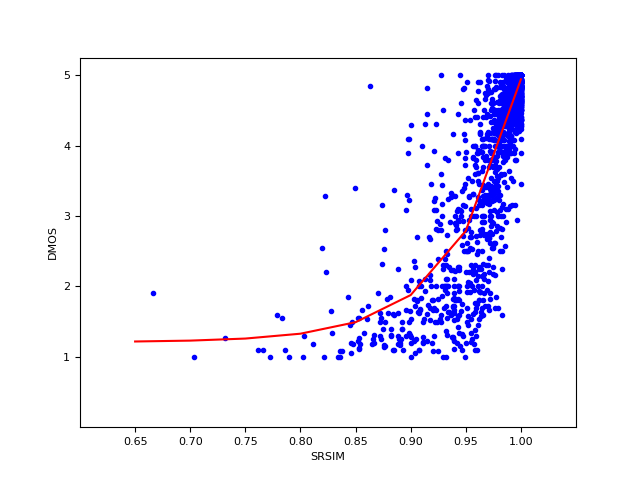
\includegraphics[width=\textwidth]{figures/srsim.png}
    \caption{SRSIM}
    \label{fig:srsim}
  \end{subfigure}%
  ~ %add desired spacing between images, e. g. ~, \quad, \qquad etc.
  %(or a blank line to force the subfigure onto a new line)
  \begin{subfigure}[b]{0.5\textwidth}
    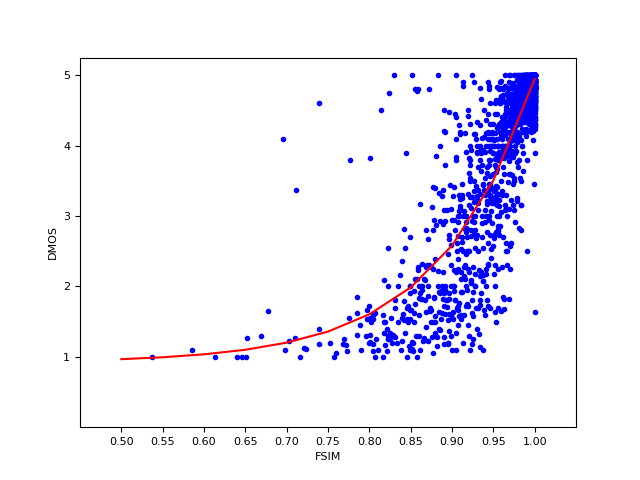
\includegraphics[width=\textwidth]{figures/fsim.png}
    \caption{FSIM}
    \label{fig:fsim}
  \end{subfigure}
  ~ %add desired spacing between images, e. g. ~, \quad, \qquad etc.
  %(or a blank line to force the subfigure onto a new line)
  \begin{subfigure}[b]{0.5\textwidth}
    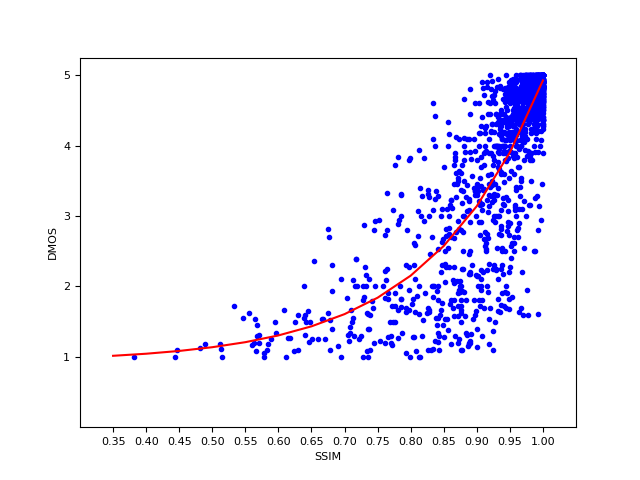
\includegraphics[width=\textwidth]{figures/ssim.png}
    \caption{SSIM}
    \label{fig:ssim}
  \end{subfigure}
  \caption{Objective Score by top 3 IQA on HMII}\label{fig:animals}
\end{figure}

From the plots, we can see that these IQA algorithms tend to predict higher score for patches. 
SRSIM and FSIM frequently predict score which is higher than $0.9_{[0-1]}$ for the image with DMOS is greater than $2_{[1-5]}$.
Although FSIM achieves highest performance with the two correlation coefficients, SSIM achieves more consistent results with subjective results on the diagrams.
These
results prove that some existing IQA models perform poorly
in distinguishing the fine-grained distortion levels, which are
feasible to determine by human visual system. Therefore, these
metrics may not be suitable for perceptual-based image compression because the distortion differences between various
coding modes are usually marginal. Moreover, the fine-grained
image-patch quality assessment is demanded and should be evaluated
on the HMII databases.

\subsection{Image-Patch Models}

In this experiment, we use the following models to evaluate with our proposed DIPQA:

\begin{itemize}
  \item \textit{IPM}: Zhang \textit{et al.}\cite{Zhang2019} assume the the curve model to predict image-patch quality is a cubic polynomial function:
  $$f(\Phi(\textbf{d});\theta) = a\Phi(\textbf{d})^{3} + b\Phi(\textbf{d})^{2} + c\Phi(\textbf{d}) + d$$
  where $\theta = {a, b, c, d}$ are the parameters for the non-linear function of Image-Patch model and $\Phi(\textbf{d})$ represents the feature of patch $\textbf{d}$. MSE and SSIM are chosen for the design of features. In our work, we tried top 3 FR-IQA methods from the first experiment: SSIM, FSIM and SRSIM.  
  
  \item \textit{DIQaM}: Bosse \textit{et al.}\cite{Bosse2018} present a Deep Neural Networks for No-Reference and Full-Reference Image Quality Assessment which obtains superior performance on different IQA benchmarks. We utilize the extractor architecture from this paper to train a Deep Neural Network on our database.
\end{itemize}

First, we use the previous works to extract the SSIM, FSIM and SRSIM feature for IPM. Then, the above curve model is fitted using the least square method to obtain the parameters that best fit the learning set. DIQaM, DIPQA (VGG extractor) and DIPQA (VGG finetuning) is built with the similar architecture which share them same regression part. With the proposed DIPQA, we approach with two different tuning strategies: one is fine-tuned with the VGGNet weight and then retrained with HMII; the other one use VGGNet as a feature extractor, this part is not trained with the entire network.
  
% Second contribution
\begin{table}[ht]
  \centering
  \begin{tabular}{|l|cc|cc|}
    \hline
    \multirow{2}{*}{} & \multicolumn{2}{c|}{ HMII (64x64) } & \multicolumn{2}{c|}{ HMII (128x128) } \\ \cline{2-5} 
    & PLCC              & SRCC            & PLCC               & SRCC             \\ \hline
    IPM (SSIM)             & 0.836             & 0.784            & 0.843              & 0.794             \\
    IPM (FSIM)             & 0.848             & 0.795            & 0.871              & 0.810             \\
    IPM (SRSIM)            & 0.854             & 0.802            & 0.857              & 0.798             \\
    DIQaM                  & 0.916             & 0.824            & 0.905              & 0.819             \\
    DIPQA (VGG extractor)  & 0.802             & 0.754            & 0.830              & 0.760             \\
    DIPQA (VGG finetuning) & \textbf{0.921}    & \textbf{0.848}   & \textbf{0.955}     & \textbf{0.871}    \\ \hline
  \end{tabular}
  \caption{Comparing different Full-Reference Image-Patch approaches}
  \label{tab:approachs}
\end{table}

The Table \ref{tab:approachs} summarizes the performance of the proposed models in comparison to other methods on HMII database in terms of PLCC and SRCC. With any of the two correlation coefficients, DIPQA (VGG finetuning) achieve superior performance to the others. From the results of this project, we can also see that the larger size of the patch seem to be more accurate when assessing image-patch quality by Objective models.